\section{Detalles de la propuesta}
En este apartado, se dará una visión global del contenido y funcionamiento de nuestra propuesta.
Se realizará una descripción completa de nuestro enfoque, desde los conceptos de \textit{IA}
empleados hasta las herramientas y tecnologías empleadas para su resolución. En primer lugar, se
detallará cómo se ha realizado la generación de los modelos, los tipos utilizados y sus
características, así como cualquier concepto relacionado. Posteriormente, se describirán las
técnicas empleadas para evaluar el rendimiento de los modelos. Continuaremos con la explicación
en detalle de las \textit{features} empleadas, qué representan y cómo se ha realizado su cálculo.
Finalmente, procederemos a explicar detalles técnicos de la implementación, como las tecnologías
y recursos empleados, el procedimiento de extracción de datos, el entorno de ejecución, etc. En
los siguientes apartados se describe con detalle cada uno de estos puntos.

\subsection{Construcción del modelo}

El Aprendizaje Automático (\textit{Machine Learning, ML})
es un campo de la Inteligencia Artificial que se centra en desarrollar algoritmos y modelos que
sean capaces de aprender y mejorar su desempeño en tareas específicas a partir de datos, sin la
necesidad de ser explícitamente programadas. Los sistemas de \textit{ML} identifican patrones en
los datos y utilizan estos patrones para hacer predicciones o tomar decisiones sobre los datos.
Podemos encontrarnos con dos tipos de aprendizaje automático:

\begin{itemize}
	\item \textbf{Supervisado}: en este tipo de aprendizaje el modelo es entrenado utilizando un
    conjunto de datos etiquetados. En este contexto ``etiquetado'' significa que cada instancia
    en el conjunto de datos viene con una entrada (conjunto de características) y una salida
    conocida (etiqueta o valor objetivo). En nuestro problema, la entrada sería el conjunto de
    características (\textit{features}) que vamos a usar y, la salida, el resultado de la
    integración continua (exitosa o fallida).
	\item \textbf{No supervisado}: en este tipo de aprendizaje el modelo es entrenado utilizando
    un conjunto de datos que no tiene etiquetas ni salidas predefinidas. A diferencia del
    supervisado, en el que se indica al modelo lo que debe predecir, en el no supervisado el
    modelo explora los datos en busca de patrones, estructuras, o relaciones ocultas.
\end{itemize}

Teniendo esto en cuenta, nos encontramos claramente ante un problema de aprendizaje supervisado,
ya que tenemos las características propias de cada \textit{build}, que sería el conjunto de
entrada que proporcionamos al modelo, y por otro lado, los resultados de las ejecuciones, que
conformarían las etiquetas o valores objetivo de nuestro problema.\\

Para poder responder a la pregunta de investigación \textbf{PI-1}, debemos explorar los
distintos algoritmos de Aprendizaje Automático que existen y ver cuál de ellos ofrece mejores
resultados en el problema que nos ocupa. En nuestro caso, nos encontramos con un claro problema
de clasificación binaria en el ámbito del aprendizaje automático supervisado. En este contexto,
tenemos dos clases posibles:
\begin{enumerate}
    \item \textbf{Clase positiva} (fallo de la \textit{build}): predicción de que la \textit{build}
    fallará.\\
    \item \textbf{Clase negativa} (éxito de la \textit{build}): predicción de que la \textit{build}
    tendrá éxito.
\end{enumerate}

Por lo tanto, dado que nos encontramos con este tipo de problema, se ha decidido utilizar seis
algoritmos de clasificación supervisada, entre los que nos encontramos:

\begin{enumerate}
    \item \textbf{Árboles de Decisión (\textit{Decision Trees, DT})}. Dividen el conjunto de datos
    en subconjuntos más pequeños y más simples, basándose en ciertas características o condiciones,
    que están representadas en un gráfico similar a un árbol. Cada nodo interno del árbol
    representa una característica (o atributo), y cada rama representa el resultado de la
    partición de los datos en función de esa característica. Las hojas del árbol contienen las
    etiquetas o valores objetivo.\\
    \item \textbf{Bosques Aleatorios (\textit{Random Forest, RF})}. Es un algoritmo de aprendizaje
    supervisado que crea un conjunto de árboles de decisión durante el entrenamiento y realiza
    la predicción promediando las predicciones de cada árbol individual. Es una técnica de
    ensamblaje que combina múltiples modelos de aprendizaje para mejorar la precisión y la
    estabilidad del modelo.\\
    \item \textbf{Regresión Logística (\textit{Logistic Regression, LR})}. Es un algoritmo de
    clasificación que se utiliza para predecir la probabilidad de que una variable dependiente
    pertenezca a una categoría particular. Aunque se llama regresión, en realidad es un algoritmo
    de clasificación binaria.\\
    \item \textbf{Máquinas de Soporte Vectorial (\textit{Support Vector Machines, SVM})}. Es un
    algoritmo de clasificación que busca encontrar el hiperplano que mejor divide un conjunto de
    datos en dos clases. El hiperplano es la línea que maximiza el margen entre las dos clases. Si
    los datos no son linealmente separables, se puede utilizar un truco matemático llamado
    \textit{kernel trick} para transformar los datos en un espacio de mayor dimensión donde sí
    sean separables.\\
    \item \textbf{Vecinos más Cercanos (\textit{K-Nearest Neighbors, KNN})}. Es un algoritmo de
    clasificación que se basa en la idea de que los puntos de datos que son similares deben
    pertenecer a la misma clase. Para predecir la clase de un nuevo punto de datos, el algoritmo
    busca los $k$ puntos de datos más cercanos en el conjunto de entrenamiento y asigna la clase
    más común entre esos vecinos.\\
    \item \textbf{Redes Neuronales (\textit{Neural Networks, NN})}. Son un conjunto de algoritmos
    de aprendizaje automático que intentan imitar el funcionamiento del cerebro humano. Consiste en
    una red de nodos interconectados, llamados neuronas, que se organizan en capas. Está formada
    por una capa de entrada, una  varias capas ocultas y una capa de salida. Cada nodo está
    conectado a los demás y tiene su propia ponderación y umbral asociados. Concretamente, se ha
    utilizado un Perceptrón Multicapa, que es un tipo de red neuronal utilizado para tareas de
    clasificación. Cada neurona en un \textit{MLP} se conecta a las de la capa anterior con pesos
    y aplica una función de activación a su suma ponderada.
\end{enumerate}

Para realizar la predicción, no únicamente se le proporciona al modelo el conjunto de
características de la \textit{build} y se predice, si no que se sigue un procedimiento más
complejo y que simula el funcionamiento de SmartBuildSkip \cite{2}. Para comprenderlo, veamos
el siguiente pseudocódigo:

\begin{algorithm}[H]
    \caption{\textit{SmartBuildSkip con nuestra implementación}}
    \begin{algorithmic}[1]
    \State \textbf{Input:} List of builds
    \State \textbf{Output:} Predictions of builds outcomes
    
    \State in\_failure\_sequence $\gets$ False \Comment{Inicializar estado de secuencia de fallos}
    \For {each build in builds}
        \If{in\_failure\_sequence}
            \State Prediction $\gets$ Fail  \Comment{Predicción automática de fallo}
            \If{build passes}               \Comment{Comprobar resultado}
                \State in\_failure\_sequence $\gets$ False \Comment{Error en la predicción, vuelve a predecir con ML}
            \EndIf
            \Else
            \State Prediction $\gets$ Machine Learning Prediction \Comment{Predicción usando ML}
            \If {Prediction = Pass}
                \State Accumulate changes with next build       \Comment{Se salta la build, acumulando cambios}
            \Else
                \If{build fails}                                \Comment{Comprobar resultado}
                    \State in\_failure\_sequence $\gets$ True   \Comment{Entra en predicción automática de fallo}
                \EndIf
            \EndIf
        \EndIf
    \EndFor
    \end{algorithmic}
\end{algorithm}

Como podemos observar, este algoritmo se divide en dos partes: una en la que predice
automáticamente que la \textit{build} fallará y otra en la que se realiza la predicción mediante
el uso de un modelo de aprendizaje automático. Esta forma de proceder es debida a las dos
hipótesis que comentamos en la Sección \ref{sec:related_work}, que muchas \textit{builds} fallan
consecutivamente después de que otra haya fallado y que las \textit{builds} exitosas siempre son
más numerosas que las fallidas. Esto hace que nuestro algoritmo pueda saltarse mayor número de
\textit{builds} a la vez que captura una mayor cantidad de \textit{build failures}.
Consecuentemente, debido a la no ejecución de estas \textit{builds}, se estará logrando una
optimización de recursos computacionales.

\subsubsection{Hiperparámetros}
Cuando se define un algoritmo de clasificación, es importante seleccionar y ajustar con cuidado
los hiperparámetros, ya que estos controlan aspectos clave del proceso de entrenamiento y pueden
determinar la capacidad del modelo para generalizar a nuevos datos. Para la definición de nuestros
algoritmos de clasificación, se ha utilizado la biblioteca \textit{scikit-learn}, una popular
biblioteca de \textit{Python} para \textit{Machine Learning} y análisis de datos. Por lo general,
se han definido todos los algoritmos con los parámetros por defecto de la biblioteca
\textit{scikit-learn}, con las siguientes particularidades:

\begin{itemize}
	\item En un conjunto de datos que contiene \textit{builds}, donde el número de \textit{builds}
    exitosas es mucho mayor que el de \textit{builds} fallidas, estamos ante un problema de
    desequilibrio de clases. En este contexto, asignar distintos pesos a las clases es una
    estrategia útil para entrenar un modelo que sea más sensible en la detección de
    \textit{builds failures}, a pesar de ser poco numerosas. Para ello, se ha definido un peso de
    20:1 a favor de las \textit{build failures} en Árbol de Decisión, Bosque Aleatorio, Regresión
    Logística y Máquinas de Soporte Vectorial.\\

	\item En Regresión Logística, se establece el número máximo de iteraciones que el algoritmo de
    optimización realizará antes de detenerse. En este caso se utiliza el valor 15.000 para
    asegurar que el algoritmo tenga suficiente tiempo para converger.\\

	\item En el algoritmo de Máquinas de Soporte Vectorial, hemos añadido el hiperparámetro que
    habilita el cálculo de probabilidades de pertenencia a cada clase. Cuando el parámetro
    \textit{probability} está habilitado, el modelo ajusta de manera interna un modelo de
    probabilidad, permitiendo que las salidas del modelo sean las etiquetas de clase y sus
    probabilidades.\\

	\item Para el Perceptrón Multicapa (redes neuronales), se ha añadido, al igual que en Regresión
    Logística, un parámetro que indica el número máximo de iteraciones para entrenar la red
    neuronal. En este caso, se ha añadido con un valor de 15000.
\end{itemize}

Además de los parámetros antes mencionados, todos ellos tienen definida la semilla de
reproducibilidad, que garantiza que los resultados sean reproducibles.

\subsection{Evaluación del modelo}
La evaluación de los modelos de clasificación tiene como objetivo medir y analizar el rendimiento
de los modelos en la tarea de clasificación. Esta evaluación permite determinar qué tan bien el
modelo puede predecir o clasificar nuevas instancias no vistas anteriormente, es decir, basándose
en un conjunto de datos de prueba. Para realizar la evaluación de los modelos en nuestro problema,
hemos seguido los siguientes pasos:

\begin{enumerate}
    \item \textbf{División del conjunto de datos}: se divide el conjunto de datos, en este caso
    \textit{features} de cada \textit{build}, en dos partes: el conjunto de entrenamiento y el
    conjunto de prueba. El conjunto de entrenamiento se utiliza para entrenar el modelo, mientras
    que el conjunto de prueba se usa para evaluar su rendimiento. Dada la naturaleza de nuestro
    problema, no podemos hacer esta división de manera aleatoria, ya que las \textit{builds} están
    relacionadas temporalmente entre sí, por lo que no sería realista realizar una predicción
    sobre una instancia antigua basándonos en \textit{builds} que se hayan ejecutado recientemente.
    Por lo tanto, en nuestro caso se ha dividido el conjunto de datos igualmente en dos partes,
    pero siendo el conjunto de entrenamiento más antiguo en su conjunto que el conjunto de prueba,
    que es más reciente. Por ejemplo si se dividen los datos de entrenamiento y test en un 80\% y
    20\% respectivamente, el conjunto de entrenamiento contendrá el 80\% de las \textit{builds}
    más antiguas, mientras que el de prueba contendrá el 20\% de \textit{builds} más reciente.\\
    \item \textbf{Predicción}: una vez entrenado el modelo con el conjunto de entrenamiento, se
    realizan predicciones sobre el conjunto de prueba. Gracias a estas predicciones, podremos
    verificar si nuestros modelos se comportan bien frente a instancias nuevas o no vistas con
    anterioridad.\\
    \item \textbf{Métricas de evaluación}: una vez realizadas las predicciones, hemos definido
    las métricas de evaluación, que nos ayudarán a determinar el rendimiento de nuestros modelos.
    Las métricas que hemos usado son: \textit{accuracy}, \textit{precision}, \textit{recall},
    \textit{F1-score}, \textit{confusion matrix} y \textit{ROC curve}. Todas
    ellas han sido descritas en la Sección \ref{sec:research_questions}, exceptuando el área
    bajo la curva \textit{ROC} (\textit{Area Under the Curve, AUC}), que mide la capacidad de
    un modelo para distinguir entre clases positivas y negativas. Cuanto mayor sea el valor de
    \textit{AUC}, mejor será el desempeño del modelo en la clasificación, ya que esta indica una
    mayor capacidad para separar correctamente las clases.
\end{enumerate}

\subsubsection{Validación Cruzada}
La validación cruzada (\textit{cross-validation}) es una técnica utilizada para la evaluación y
selección de modelos, midiendo su rendimiento y capacidad de generalización. Su objetivo
principal es evitar el sobreajuste (\textit{overfitting}), que ocurre cuando un modelo
aprende demasiado de los datos de entrenamiento y es incapaz de generalizar a nuevos datos. Esta
consiste en dividir el conjunto de datos en $k$ subconjuntos (\textit{folds}), entrenar el modelo
en $k-1$ subconjuntos y evaluarlo en el subconjunto restante. Este proceso se repite $k$ veces,
de forma que cada subconjunto se utiliza una vez como conjunto de prueba. Al final, se promedian
los resultados de las $k$ iteraciones para obtener una estimación más precisa del rendimiento del
modelo.\\

En nuestro caso particular, hemos tenido que hacer una ligera variación de esta técnica. En
nuestro problema, la división del conjunto de datos en $k$ subconjuntos no puede realizarse de
manera aleatoria, ya que no tendría sentido realizar predicciones para instancias más antiguas
utilizando para el entrenamiento instancias más recientes. Es decir, en nuestro problema existe
una dependencia temporal y, por tanto, la secuencia y el orden de los datos son críticos para la
validez de las predicciones. Los resultados y características de las \textit{builds} están
influenciados por las \textit{builds} anteriores. Esto se debe a que cada \textit{build} puede
depender de cambios de código, configuraciones, y otros factores que se acumulen o evolucionen
con el tiempo. Por lo tanto, si se permite que las \textit{builds} más antiguas predigan utilizando
información de \textit{builds} más recientes, se introduciría un sesgo temporal que no reflejaría
el comportamiento real del sistema. Además de esto, usar datos de \textit{builds} futuras para
predecir \textit{builds} antiguas no solamente introduce un sesgo, si no que también puede dar
una falsa impresión de precisión del modelo, llevando a resultados artificialmente inflados de
precisión durante esta fase de evaluación.\\

En nuestra implementación dividimos el conjunto en 11 partes de forma secuencial, de modo que el
primer subconjunto contenga las \textit{builds} más antiguas y el último las \textit{builds} más
recientes. El subconjunto de \textit{folds} se recorre y en cada iteración, se entrena con la
acumulación de subconjuntos anteriores, y se evalúa con el siguiente subconjunto, dejando el resto
de subconjuntos sin utilizar. Siempre que se tengan $k$ \textit{folds} se realizarán $k-1$
iteraciones, ya que en la última iteración se utilizará el último subconjunto como conjunto de
prueba. Finalmente, dado que se habrán obtenido 10 resultados de las métricas de evaluación, se
promedian para obtener una estimación más precisa del rendimiento del modelo.\\

A continuación, se presenta de forma gráfica el funcionamiento de nuestro algoritmo de
\textit{key-fold cross validation}:

\begin{figure}[H]
    \centering
    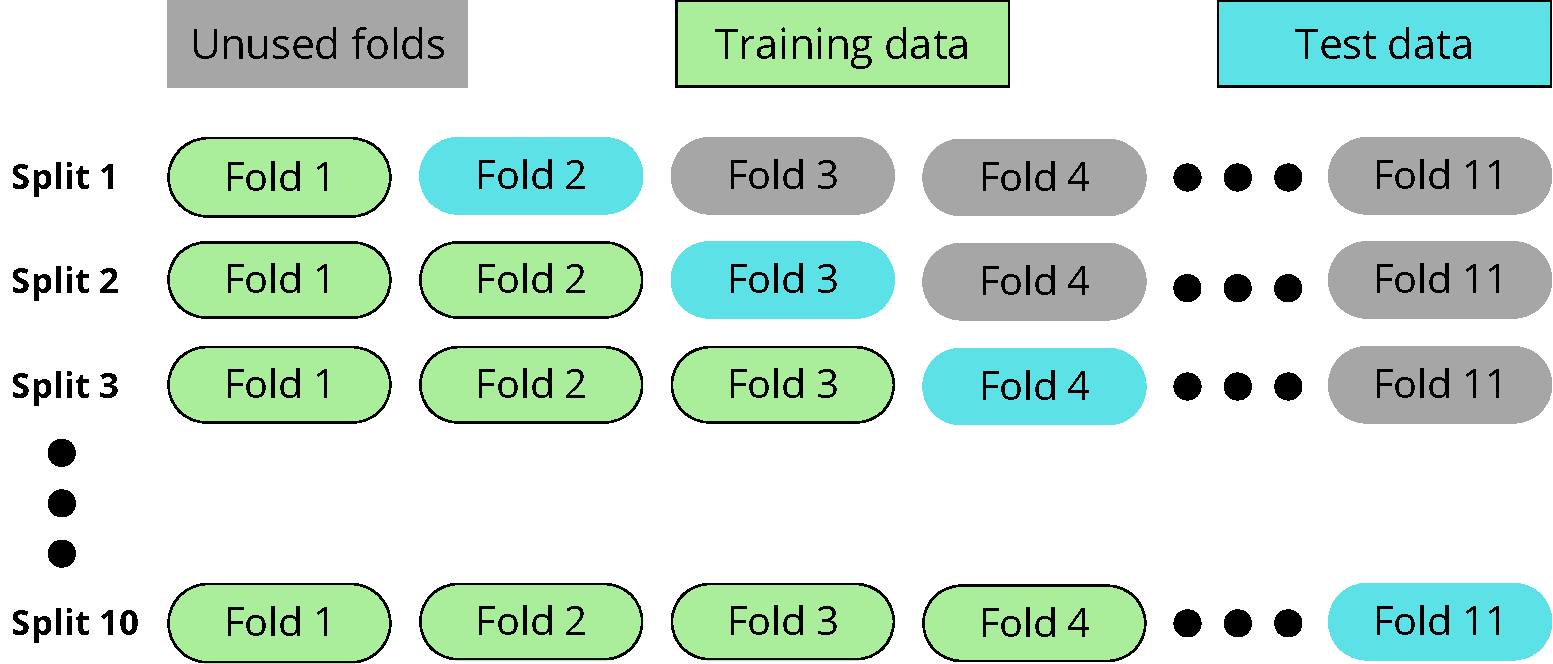
\includegraphics[scale=0.5]{images/Cross validation.pdf}
    \caption{Funcionamiento de la técnica \textit{key-fold cross validation}.}
    \label{fig:confusion_matrix}
\end{figure}

\subsubsection{Umbral de decisión}
La evaluación de los modelos a distintos grados de sensibilidad es especialmente relevante cuando
se consideran problemas de clasificación con clases desbalanceadas o cuando el costo de los
errores varían entre clases. En el problema que nos ocupa, se dan ambas condiciones: por lo
general, el número de \textit{builds} exitosas es muy superior al de \textit{builds} fallidas y,
el costo de predecir un falso negativo no es el mismo que el de predecir un falso positivo. Al
ajustar la sensibilidad del modelo, se balancean las tasas de verdaderos positivos
(\textit{recall}) y falsos positivos, lo que permite optimizar el rendimiento del modelo para
diferentes contextos y necesidades.\\

Muchos algoritmos de aprendizaje automático pueden predecir una probabilidad de
pertenencia a una clase. Esto es útil porque proporciona una medida de la certeza o incertidumbre
de una predicción y ofrece más detalles que solo predecir la etiqueta de la clase. En nuestro
problema, es necesario convertir estas probabilidades en el valor de una clase. Esta conversión
se basa en un parámetro llamado ``umbral de decisión''. El valor por defecto de este umbral
es $0.5$ para probabilidades normalizadas en el intervalo $[0, 1]$. Por ejemplo, dadas las
etiquetas de nuestro problema: $0$ (la \textit{build} falla) y $1$ (la \textit{build} pasa), si
la probabilidad de que una \textit{build} falle es igual o mayor a $0.5$, se predecirá que la
\textit{build} es exitosa, mientras que si es menor a $0.5$, se predecirá que la \textit{build}
falla.\\

En nuestra implementación, hemos evaluado el rendimiento de todos los modelos y variantes del
mismo para valores del umbral de decisión comprendidos en el intervalo $[0, 1]$. Para ello, se
han calculado las métricas de evaluación para cada valor del umbral y se han representado en
gráficos para poder comparar el rendimiento de los modelos en función del umbral de decisión. De
esta forma, se ha podido determinar cuál de ellos es el que mejor rendimiento ofrece y cuál de
las implementaciones es la que mejor resultado proporciona.


\subsection{\textit{Features} empleadas}
Las \textit{features} o características son las propiedades o atributos que se utilizan como entrada
para entrenar un modelo. Son elementos fundamentales que permiten al modelo aprender patrones y
tomar decisiones basadas en los datos. Las \textit{features} recogen información relevante de
los datos, en este caso de las \textit{builds}. La calidad y relevancia de las mismas afecta
al rendimiento del modelo, por lo que escoger las adecuadas es fundamental. Al hacer la selección
de las \textit{features}, hay que tener en cuenta lo siguiente:

\begin{itemize}
    \item Elegir \textit{features} que sean relevantes y representativas del problema es importante
    para que el modelo sea preciso y eficiente. Además, ayuda a reducir la dimensionalidad
    del problema, lo que puede mejorar la eficiencia computacional y la interpretabilidad del
    modelo.\\
    \item Seleccionar gran cantidad de \textit{features} puede llevar a un sobreajuste del modelo,
    donde el modelo aprende de patrones de datos ruidosos o irrelevantes. Esto puede llevar a un
    rendimiento bajo y a modelos menos generalizables
\end{itemize}

\noindent A continuación, se presentan las features empleadas en nuestro problema.

\begin{table}[h]
    \centering
    \caption{\textit{Build features} empleadas.}
    \label{tab:features}

    \begin{tabular}{|>{\centering\arraybackslash}m{4cm}|>{\centering\arraybackslash}m{8cm}|} % Encabezados centrados
        \hline
        \textbf{\textit{Feature}} & \textbf{Descripción breve} \\
        \hline
    \end{tabular}
    \begin{tabular}{|>{\raggedright\arraybackslash}m{4cm}|>{\raggedright\arraybackslash}m{8cm}|} % Contenido alineado a la izquierda en la esquina superior
        \hline
        \textbf{\textit{Performance Short} (PS)\footnote{\textit{Build feature propuesta en \cite{2} pero que finalmente no se usó en el mismo.}}} & La proporción de \textit{builds} exitosas en las últimas cinco \textit{builds}.\\
        \hline
        \textbf{\textit{Performance Long} (PL)\footnotemark[1]} & La proporción de \textit{builds} exitosas de todas las \textit{builds} previas.\\
        \hline
        \textbf{\textit{Time Frequency} (TF)\footnotemark[1]} & El intervalo de tiempo en horas desde la última \textit{build}.\\
        \hline
        \textit{Number Commits} (NC) & El número de \textit{commits desde la última \textit{build}.}\\
        \hline
        \textit{Files Changed} (FC) & El número de archivos modificados desde la última \textit{build}, incluyendo archivos añadidos, modificados y eliminados.\\
        \hline
        \textbf{\textit{Files Added} (FA)} & El número de archivos añadidos desde la última \textit{build}.\\
        \hline
        \textbf{\textit{Files Modified} (FM)} & El número de archivos modificados desde la última \textit{build}.\\
        \hline
        \textbf{\textit{Files Removed} (FR)} & El número de archivos modificados desde la última \textit{build}.\\
        \hline
        \textit{Source Lines Changed} (LC) & El número de líneas de código modificadas desde la última \textit{build}, incluyendo líneas añadidas y eliminadas.\\
        \hline
        \textbf{\textit{Source Lines Added} (LA)} & El número de líneas de código añadidas desde la última \textit{build}.\\
        \hline
        \textbf{\textit{Source Lines Removed} (LR)} & El número de líneas de código eliminadas desde la última \textit{build}.\\
        \hline
        \textit{Test Lines Changed} (LT) & El número de líneas de código de \textit{test} modificadas desde la última \textit{build}, incluyendo líneas añadidas y eliminadas.\\
        \hline
        \textbf{\textit{Unit Tests} (UT)} & Si se han escrito pruebas unitarias desde la última \textit{build}.\\
        \hline
        \textbf{\textit{Failure Distance} (FD)\footnotemark[1]} & El número de \textit{builds} exitosas desde la última \textit{build} fallida.\\
        \hline
        \textbf{\textit{Week Day} (WD)\footnotemark[1]} & El día de la semana en el que se ha ejecutado la \textit{build}.\\
        \hline
        \textbf{\textit{Day Hour} (DH)\footnotemark[1]} & La hora del día en la que se ha ejecutado la \textit{build}.\\
        \hline
        \textbf{\textit{Commit Delay} (CD)} & El tiempo transcurrido en horas entre \textit{commits} de una misma \textit{build}.\\
        \hline
        % Añade más filas según sea necesario
    \end{tabular}
\end{table}
\footnotetext{\textit{Build feature propuesta en SmartBuildSkip pero que finalmente no se usó para el entrenamiento del modelo \cite{2}}.}

Las \textit{features} marcadas en negrita son \textit{features} nuevas propuestas en este trabajo
para realizar el entrenamiento de los modelos, mientras las que no están marcadas en negrita son
\textit{features} propuestas y utilizadas en estudios previos \cite{2}.\\

\noindent Para el cálculo de las \textit{features} mencionadas en la Tabla \ref{tab:features},
debemos tener en cuenta los siguientes aspectos:

\begin{itemize}
    \item \textbf{Información para el entrenamiento}: cuando obtenemos las características de las \textit{builds}
    directamente desde el repositorio de código fuente, tenemos acceso a la información completa
    de cada una de ellas. El cálculo de las \textit{features} es sencillo y directo, ya que
    podemos acceder a la información de cada \textit{build} que se ha ejecutado y extraer las
    características necesarias.\\
    
    \item \textbf{Cálculo de Features durante la predicción}: debemos recordar que, en el
    enfoque que planteamos, a veces no se ejecutan todas las \textit{builds} que se han
    programado. Por lo tanto, no siempre se tiene acceso a la información real (\textit{Ground
    Truth}) de haber ejecutado las \textit{builds}. \textit{Features} como el \textit{performance
    short}, el \textit{performance long} o el \textit{failure distance} deben ser calculadas
    de forma diferente para poder simular un comportamiento práctico real.\\

    \item \textbf{Normalización}: es importante normalizar las \textit{features} antes de
    entrenar el modelo. La normalización es un proceso que ajusta los valores de las
    \textit{features} para que tengan una escala común. Esto es importante porque muchos
    algoritmos de aprendizaje automático son sensibles a la escala de las \textit{features} y
    pueden dar resultados incorrectos si las \textit{features} tienen escalas muy diferentes.\\
\end{itemize}

\subsubsection*{Cáculo de \textit{features} durante la predicción}. Para comprender bien este
punto, vamos a diferenciar dos conceptos fundamentales: la \textbf{\textit{build} propuesta} y la
\textbf{\textit{build} ejecutada}. La \textit{build} propuesta es aquella que se desea predecir,
independientemente de lo que prediga el algoritmo de predicción, y que por lo tanto todavía no ha
sido ejecutada. La \textit{build} ejecutada es aquella que previamente era una \textit{build}
propuesta (a predecir) y que ha sido ejecutada porque el algoritmo predijo que fallaría. Teniendo
claros estos dos conceptos, pasemos a la explicación del cálculo de las \textit{features}
mencionadas anteriormente:

\begin{itemize}
    \item \textbf{\textit{Performance Short} (PS)}: para calcular este porcentaje de \textit{builds}
    exitosas en las últimas cinco \textit{builds}, cuando el algoritmo predice que la \textit{build}
    propuesta pasará, se salta la ejecución de la \textit{build} y se asume que el algoritmo ha
    acertado. Cuando el algoritmo predice que la \textit{build} propuesta fallará, la \textit{build}
    se ejecutará y, podremos ver el resultado real de la \textit{CI}, considerando dicho valor.\\

    \item \textbf{\textit{Performance Long} (PL)}: al igual que en el caso anterior, se calcula el
    porcentaje de \textit{builds} exitosas de todas las \textit{builds} propuestas hasta el momento.
    Si el algoritmo predice que la \textit{build} propuesta pasará, se asume que ha acertado y si
    predice que fallará, se ejecuta la \textit{build} y se considera el resultado real.\\

    \item \textbf{\textit{Failure Distance} (FD)}: se calculará como el número de \textit{builds}
    exitosas desde la última \textit{build} fallida. Si el algoritmo predice que la \textit{build}
    propuesta pasará, se asume que ha acertado y si predice que fallará, se ejecuta la
    \textit{build} y se considera el resultado real.\\

\end{itemize}

\noindent A continuación, se representa de forma gráfica el cálculo de cada uno de ellos:

\begin{figure}[H]
    \centering
    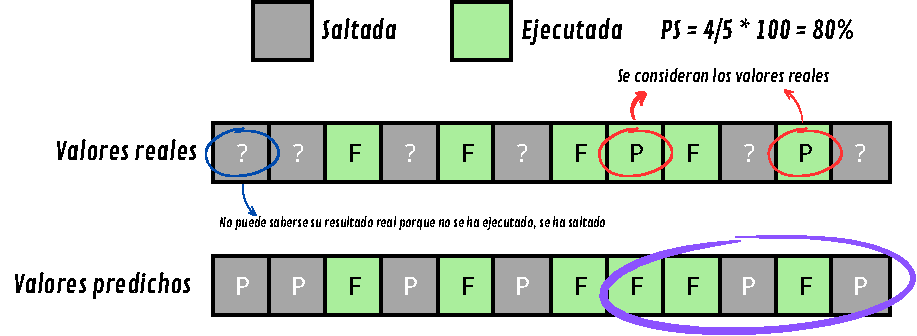
\includegraphics[scale=0.9]{images/PS.pdf}
    \caption{Cáculo del \textit{Performance Short}.}
    \label{fig:PL}
\end{figure}

\begin{figure}[H]
    \centering
    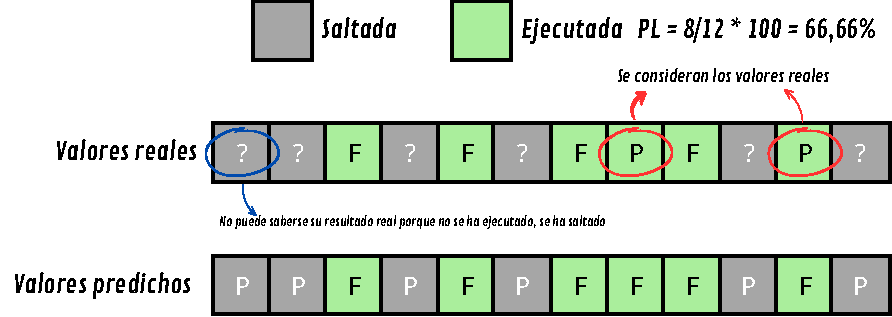
\includegraphics[scale=0.9]{images/PL.pdf}
    \caption{Cáculo del \textit{Performance Long}.}
    \label{fig:PL}
\end{figure}

\begin{figure}[H]
    \centering
    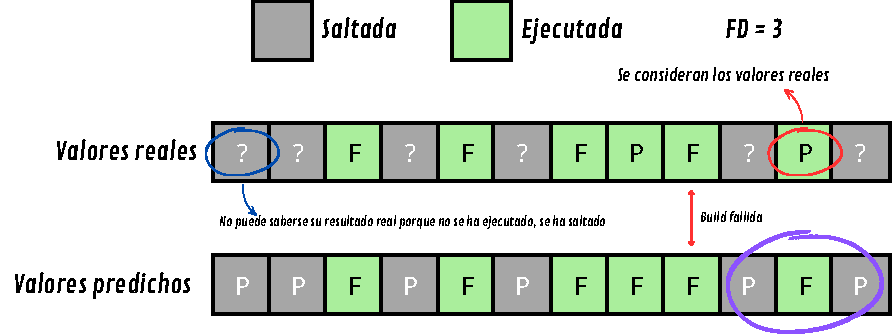
\includegraphics[scale=0.9]{images/FD.pdf}
    \caption{Cáculo del \textit{Failure Distance}.}
    \label{fig:PL}
\end{figure}

\subsection{Interfaz gráfica}


\subsection{Detalles técnicos de la implementación}

